\chapter{About the evaluated tools}
\label{chap:tools}

This chapter provides elaborate descriptions of the evaluated tools and information about the proof-of-concept implementations. 

\section{Apache Cordova}

\subsection{General information \& history}

Apache Cordova\footnote{\url{http://cordova.apache.org}} started out as a project called PhoneGap. It was developed by a couple of employees from a Canadian company called Nitobi and was unofficially released at the iPhoneDevCamp gathering in August 2008. In 2011, Adobe acquired said company such that the team could focus solely on the development of PhoneGap. At the same time, Nitobi donated the PhoneGap codebase to the Apache Software Foundation (ASF), where it became an incubating\footnote{In order to become part of the ASF, every project is required to go through an incubating stage.} project. To make sure that the intellectual property would not conflict with trademark ambiguity, the project's name was changed from PhoneGap to Apache Callback. Because the community was dissatisfied with the project's name, it was quickly changed to Apache Cordova. On October 2012, Apache Cordova graduated as a top level project within the Apache Software Foundation. This ensures that it will always remain free and open source under the Apache License 2.0.

Nowadays, PhoneGap is a distribution of Apache Cordova, delivered by Adobe, while development and open source contributions happen in the Apache Cordova project. PhoneGap strategically fits in a collection of software like Adobe PhoneGap Build and Adobe Edge Inspect. 

\subsection{Supported platforms}
\label{sec:ac:support}

Apache Cordova supports a large number of platforms, both mobile and non-mobile.
\begin{itemize}
    \item The current release supports Android (2.1 and up), iOS (4 and up), BlackBerry (5 and up), Windows Phone (7 and 8) and Windows (7 and 8). 
    \item Future releases of Cordova are likely to support for Tizen, Qt, Firefox OS, Ubuntu Mobile.
    \item Support for Symbian, Bada and WebOS is decreasing as these platforms are considered to be dying. 
\end{itemize}

\subsection{Architecture}
\label{sec:cordova:architecture}

Apache Cordova is a cross-platform tool that produces hybrid applications, i.e. the actual application is a mobile web application. This web application is wrapped inside a native shell which provides access to the hardware through a JavaScript bridge. This architecture is visualized in \fref{fig:cordova:architecture}. Wrapping an application can be either done locally or through a building service in the cloud called Adobe PhoneGap Build.

\begin{figure}
    \begin{center}
        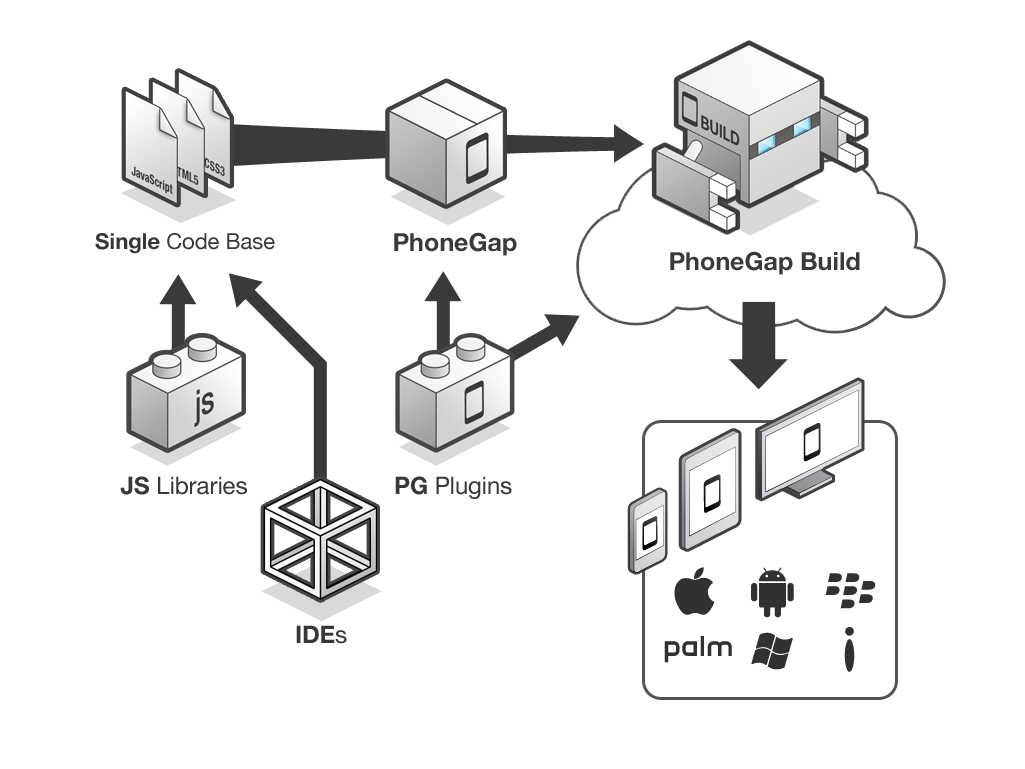
\includegraphics[width=.8\textwidth]{figs/cordova-architecture.png}
        \caption{The architecture of Apache Cordova / Adobe PhoneGap applications.}
        \label{fig:cordova:architecture}
    \end{center}
\end{figure}

One of Cordova's goals is to promote the web as a first-class development platform. However, many mobile browser implementations are still lacking decent HTML5 support. Cordova solves this problem by providing HTML5 polyfills for these browsers. A polyfill is a sort of plugins that addresses the lack of a specific feature in a browser. The API of the polyfill typically matches the official API such that applications do not notice that the feature is missing. If the browser does have support for a particular feature, the browsers implementation is used. 

\paragraph{Example} The Cordova Storage API is a polyfill for the deprecated but often used Web SQL specification\footnote{\url{http://dev.w3.org/html5/webdatabase/}} and Web Storage specification\footnote{\url{http://dev.w3.org/html5/webstorage/}}. 

\subsubsection{Plugin system}

Within Cordova, every device API is implemented as a plugin. This allows to (1) leave out unused device API's, reducing the size of the compiled application and (2) create your own custom plugin. Every plugin comprises of a piece of JavaScript code and a piece of native code. Calls to the JavaScript API are marshaled and sent to the native counterpart where the request gets unmarshaled and executed. Additionally, a response is be sent back to the caller.

A comprehensive list of Cordova plugins is available at \url{https://github.com/phonegap/phonegap-plugins}. However, at the time of writing, there is no package manager like \texttt{npm}\footnote{NPM is the Node Package Manager, \url{http://npmjs.org}} available for Cordova plugins.

\subsection{Related projects}

There are a number of projects related to Apache Cordova that are useful when developing mobile web applications with Cordova.

\subsubsection{Adobe PhoneGap Build}

Adobe PhoneGap Build\footnote{\url{http://build.phonegap.com}}, part of Adobe Edge Tools \& Services, is an online build service for packaging Cordova/PhoneGap applications. Upon request, the application's source code is pulled from a git\footnote{Git is a popular version control system, \url{http://git-scm.org}} repository and the packaged app can be downloaded straight from the web interface. An API is available to automate the process. The service supports Android, iOS, Windows Phone, BlackBerry, WebOS and Symbian.

Both free and paid plans (with a monthly subscription fee) are available. The free plan is entitled to only one private project, a paid plan is entitled to 25 or more private apps.

\subsubsection{Edge Inspect}

Another Adobe product is called Edge Inspect\footnote{\url{http://html.adobe.com/edge/inspect/}}, which is also part of Adobe Edge Tools \& Services. It comprises of a desktop application, a Chrome plugin and a couple of native applications and allows developers to preview web designs on multiple displays at a time. When the plugin is activated, all connected devices instantly load the same web page. At the same time, developers get access to a WebKit inspector, showing the code of any remote browser (this is based on WEINRE, see further). The application also allows the developer to take screen shots the web pages displayed in a particular browser.

\subsubsection{WEINRE}

WEINRE\footnote{\url{http://people.apache.org/~pmuellr/weinre/docs/latest/}} is part of Apache Cordova and is an acronym for ``WEb INspector REmote''. It provides access to a fully functional WebKit inspector of remote browsers. The service runs on a node\footnote{Server-side JavaScript, \url{http://nodejs.org}} server. The only requirement is to include a javascript file in the application's HTML. When the browser starts executing the JavaScript file, it makes a persistent connection with a server through a web socket. This connection is then used for all communication between the web application and the WebKit inspector. This allows developers to inspect the DOM, resources, run custom JavaScript commands, etc. remotely.

A hosted version is available at \url{http://debug.phonegap.com}.

\subsubsection{Apache Ripple}

Apache Ripple\footnote{\url{http://ripple.incubator.apache.org}} is a web-based mobile environment simulator and is available as a Chrome extension. It exposes the Apache Cordova device API's and allows developers to simulate various device features in a desktop browser. For instance, you can shake the device, set a location and heading, emulate disruptive networking, etc.

\subsection{Proof-of-concept application implementation}

This subsection provides an overview and short description of the technologies that were used to implement the proof-of-concept application. 

The proof-of concept application is implemented as a single-page application. This eliminates page loads and thus improves overall performance of the application. The application code is all wrapped inside the native shell. Instead, future versions could serve application code from a remote server and use AppCache to cache the application data on the device. This way, the application can receive updates without the need of updating the outer shell. The application logic is built with AngularJS, the user interface is built on top of Bootstrap 3. The development workflow is based on Yeoman, which provides useful tools for scaffolding, building, previewing, testing, etc. Unit and integration tests are created with the Jasmine test framework and run with the Karma test runner.

\subsubsection{AngularJS}

AngularJS\footnote{\url{http://angularjs.org}} is an JavaScript MVC application framework, developed at Google. With AngularJS, developers can use a declarative programming style rather than an imperative style. This is achieved through additional HTML elements and attributes, which serve as annotations. In addition, the imperative programming style is still available to program controller code. AngularJS also provides a dependency injection system which makes testing so much easier. Components that require user interaction or are not useful in a testing environment can easily be replaced with a mock.

AngularJS has proven useful from the start. The project came to live at Google because developers of the Google Feedback project were unsatisfied with the development speed. The project that already took 6 months to create and 1700 lines of traditional HTML and JavaScript could be completely rewritten in three weeks by a single individual and with only 1500 lines of code \cite{Green:2013}.

\subsubsection{Bootstrap 3}

Bootstrap\footnote{\url{http://getbootstrap.com}} is a popular html user interface framework. Version 3 is a complete overhaul of the project, introducing a mobile-first approach. Instead of scaling down desktop pages, the new version starts from the mobile interface and scales up as the screen size increases. 

\subsubsection{Yeoman}

Yeoman\footnote{\url{http://yeoman.io}} is a collection of tools and best practices to make web development easier. It is comprised of the following tools:
\begin{itemize}
    \item \textbf{Yo} This command-line tool is used for scaffolding application code. A Yo plugin for AngularJS projects is available at \url{https://github.com/yeoman/generator-angular} and can generate various application artifacts.
    \item \textbf{Grunt} This command-line tool is similar to make\footnote{\url{https://www.gnu.org/software/make/}} and runs various predefined JavaScript tasks like compiling LESS files, minifying javascript and CSS, linting Javascript, running unit tests, etc.
    \item \textbf{Bower} This command-line tool is a package manager for web applications and takes care of hard to track dependencies in complex projects. 
\end{itemize}

\subsubsection{Jasmine \& Karma}

One of AngularJS' focal points is writing testable code. The community has created a test runner, called Karma\footnote{\url{http://karma-runner.github.io/}}. Running Karma will start a basic server, open a collection of browser windows (even mobile browser on connected devices or a headless browser like PhantomJS\footnote{\url{http://phantomjs.org/}}) and run all the tests in these browsers. The results of the tests are then passed back to the test runner in order to report them to the user. 

The tests are coded with the Jasmine\footnote{\url{http://pivotal.github.io/jasmine/}} testing framework.

\section{Motorola Rhodes}

\subsection{Architecture}

\TODO{Rhodes is an interpreted/hybrid application, uses ruby and HTML(5) for ui but has no support for HTML5 polyfills if browser support is limited, ...}

\TODO{Elaborate description of Rhodes, including architecture, kind of app, supported platforms, used programming languages, costs, financial backing, community support, official support, ...}

\section{Native SDKs?}